\documentclass[a4paper]{article}
\usepackage{geometry}
\usepackage{graphicx}
\usepackage{natbib}
\usepackage{amsmath}
\usepackage{amssymb}
\usepackage{amsthm}
\usepackage{paralist}
\usepackage{epstopdf}
\usepackage{tabularx}
\usepackage{longtable}
\usepackage{multirow}
\usepackage{multicol}
\usepackage{hyperref}
\usepackage{fancyvrb}
\usepackage{algorithm}
\usepackage{algorithmic}
\usepackage{float}
\usepackage{paralist}
\usepackage[svgname]{xcolor}
\usepackage{enumerate}
\usepackage{array}
\usepackage{times}
\usepackage{url}
\usepackage{fancyhdr}
\usepackage{comment}
\usepackage{environ}
\usepackage{times}
\usepackage{textcomp}
\usepackage{caption}
\usepackage{color}
\usepackage{xcolor}

\urlstyle{rm}

\setlength\parindent{0pt} % Removes all indentation from paragraphs
\theoremstyle{definition}
\newtheorem{definition}{Definition}[]
\newtheorem{conjecture}{Conjecture}[]
\newtheorem{example}{Example}[]
\newtheorem{theorem}{Theorem}[]
\newtheorem{lemma}{Lemma}
\newtheorem{proposition}{Proposition}
\newtheorem{corollary}{Corollary}

\floatname{algorithm}{Procedure}
\renewcommand{\algorithmicrequire}{\textbf{Input:}}
\renewcommand{\algorithmicensure}{\textbf{Output:}}
\newcommand{\abs}[1]{\lvert#1\rvert}
\newcommand{\norm}[1]{\lVert#1\rVert}
\newcommand{\RR}{\mathbb{R}}
\newcommand{\CC}{\mathbb{C}}
\newcommand{\Nat}{\mathbb{N}}
\newcommand{\br}[1]{\{#1\}}
\DeclareMathOperator*{\argmin}{arg\,min}
\DeclareMathOperator*{\argmax}{arg\,max}
\renewcommand{\qedsymbol}{$\blacksquare$}

\definecolor{dkgreen}{rgb}{0,0.6,0}
\definecolor{gray}{rgb}{0.5,0.5,0.5}
\definecolor{mauve}{rgb}{0.58,0,0.82}

\newcommand{\Var}{\mathrm{Var}}
\newcommand{\Cov}{\mathrm{Cov}}

\newcommand{\vc}[1]{\boldsymbol{#1}}
\newcommand{\xv}{\vc{x}}
\newcommand{\Sigmav}{\vc{\Sigma}}
\newcommand{\alphav}{\vc{\alpha}}
\newcommand{\muv}{\vc{\mu}}

\newcommand{\red}[1]{\textcolor{red}{#1}}

\def\x{\mathbf x}
\def\y{\mathbf y}
\def\w{\mathbf w}
\def\v{\mathbf v}
\def\E{\mathbb E}
\def\V{\mathbb V}

% TO SHOW SOLUTIONS, include following (else comment out):
\newenvironment{soln}{
    \leavevmode\color{blue}\ignorespaces
}{}


\hypersetup{
%    colorlinks,
    linkcolor={red!50!black},
    citecolor={blue!50!black},
    urlcolor={blue!80!black}
}

\geometry{
  top=1in,            % <-- you want to adjust this
  inner=1in,
  outer=1in,
  bottom=1in,
  headheight=3em,       % <-- and this
  headsep=2em,          % <-- and this
  footskip=3em,
}


\pagestyle{fancyplain}
\lhead{\fancyplain{}{Homework 2}}
\rhead{\fancyplain{}{CS 760 Machine Learning}}
\cfoot{\thepage}

\title{\textsc{Homework 2}} % Title

%%% NOTE:  Replace 'NAME HERE' etc., and delete any "\red{}" wrappers (so it won't show up as red)

\author{
Ivan Hu \\
9081641624\\
}

\date{}

\begin{document}

\maketitle


\textbf{Instructions:}
Use this latex file as a template to develop your homework. Submit your homework on time as a single pdf file to Canvas. Please wrap your code and upload to a public GitHub repo, then attach the link below the instructions so that we can access it. You can choose any programming language (i.e. python, R, or MATLAB), as long as you implement the algorithm from scratch (e.g. do not use sklearn on questions 1 to 7 in section 2). Please check Piazza for updates about the homework.

\begin{soln}
  Code is located at: \href{https://github.com/ivanlhu/cs760-hw2}{https://github.com/ivanlhu/cs760-hw2}
\end{soln}

\section{A Simplified Decision Tree}
You are to implement a decision-tree learner for classification.
To simplify your work, this will not be a general purpose decision tree.  Instead, your program can assume that
\begin{itemize}
\item each item has two continuous features $\x \in \RR^2$
\item the class label is binary and encoded as $y \in \{0,1\}$
\item data files are in plaintext with one labeled item per line, separated by whitespace:
$$x_{11} \quad x_{12} \quad y_1$$
$$...$$
$$x_{n1} \quad x_{n2} \quad y_n$$
\end{itemize}

Your program should implement a decision tree learner according to the following guidelines:
\begin{itemize}
\item Candidate splits $(j,c)$ for numeric features should use a threshold $c$ in feature dimension $j$ in the form of $x_{j}\ge c$.
\item $c$ should be on values of that dimension present in the training data; i.e. the threshold is on training points, not in between training points. You may enumerate all features, and for each feature, use all possible values for that dimension.
\item You may skip those candidate splits with zero split information (i.e. the entropy of the split), and continue the enumeration.
\item The left branch of such a split is the ``then'' branch, and the right branch is ``else''.
\item Splits should be chosen using information gain ratio. If there is a tie you may break it arbitrarily.
\item The stopping criteria (for making a node into a leaf) are that
	\begin{itemize}
	\item the node is empty, or
	\item all splits have zero gain ratio (if the entropy of the split is non-zero), or
	\item the entropy of any candidates split is zero
	\end{itemize}
\item To simplify, whenever there is no majority class in a leaf, let it predict $y=1$.
\end{itemize}

\section{Questions}
\begin{enumerate}
  \item (Our algorithm stops at pure labels) [10 pts] If a node is not empty but contains training items with the same label, why is it guaranteed to become a leaf?  Explain. You may assume that the feature values of these items are not all the same. \\

        \begin{soln}
          If all items have the same label, then every candidate split will give them the same class label. This means that the entropy of every candidate split is zero, which is a stopping criterion for the node.
        \end{soln}

\item (Our algorithm is greedy)  [10 pts] Handcraft a small training set where both classes are present but the algorithm refuses to split; instead it makes the root a leaf and stop;
Importantly, if we were to manually force a split, the algorithm will happily continue splitting the data set further and produce a deeper tree with zero training error.
        You should (1) plot your training set, (2) explain why.  Hint: you don't need more than a handful of items. \\
        \begin{soln}
          Consider the dataset with points $\x=(0,0),(1,1)$ assigned with $y=0$, and $\x=(0,1),(1,0)$ assigned with $y=1$.


          \begin{center}
            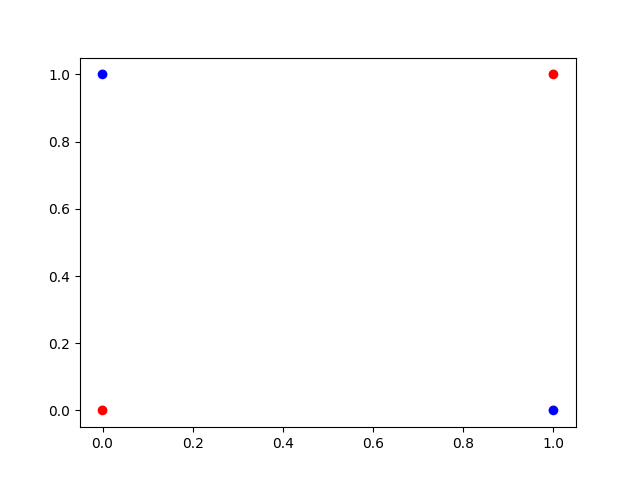
\includegraphics[width=0.6\linewidth]{p2.png}
          \end{center}


          The only nontrivial candidate splits are $S_{1}=x_{1}\ge 1$ and $S_{2}=x_{2}\ge 1$. We can compute that $H(Y)=1$, $H(Y|S_{1})=1$, and $H(Y|S_{2})=1$, since in each scenario $y=0$ and $y=1$ both have $1/2$ probability. As a result, both $S_{1}$ and $S_{2}$ have info gain ratio of 0, meaning that the algorithm will not make any split.

          However, if we forced split $S_{1}$, then for the $x_{1}\ge 1$ branch, the algorithm will make another split: $x_{2}\ge 1\implies y=0$ and $x_{2}<1\implies y=1$; for the $x_{1}<1$ branch, the algorithm will make the split $x_{2}\ge 1\implies y=1$ and $x_{2}<1\implies y=0$. This classifies the training data with zero error.
        \end{soln}


  \item (Information gain ratio exercise)  [10 pts] Use the training set Druns.txt.  For the root node, list all candidate cuts and their information gain ratio. If the entropy of the candidate split is zero, please list its mutual information (i.e. information gain). Hint: to get $\log_2(x)$ when your programming language may be using a different base, use \verb|log(x)/log(2)|. Also, please follow the split rule in the first section. \\

        \begin{soln}
          Output of \verb|p3()|:

\begin{verbatim}
Candidate split x_1 >= 0.100:
    Gain ratio: 0.101

Candidate split x_1 >= 0.000:
    Split has no entropy
    Split has information gain 0.000

Candidate split x_2 >= 0.000:
    Gain ratio: 0.056

Candidate split x_2 >= 1.000:
    Gain ratio: 0.006

Candidate split x_2 >= 2.000:
    Gain ratio: 0.001

Candidate split x_2 >= 3.000:
    Gain ratio: 0.016

Candidate split x_2 >= 4.000:
    Gain ratio: 0.050

Candidate split x_2 >= 5.000:
    Gain ratio: 0.111

Candidate split x_2 >= 6.000:
    Gain ratio: 0.236

Candidate split x_2 >= 7.000:
    Gain ratio: 0.056

Candidate split x_2 >= 8.000:
    Gain ratio: 0.430

Candidate split x_2 >= -1.000:
    Gain ratio: 0.101

Candidate split x_2 >= -2.000:
    Split has no entropy
    Split has information gain 0.000
\end{verbatim}

        \end{soln}

\item (The king of interpretability)  [10 pts] Decision tree is not the most accurate classifier in general.  However, it persists.  This is largely due to its rumored interpretability: a data scientist can easily explain a tree to a non-data scientist.  Build a tree from D3leaves.txt.  Then manually convert your tree to a set of logic rules.  Show the tree\footnote{When we say show the tree, we mean either the standard computer science tree view, or some crude plaintext representation of the tree -- as long as you explain the format.  When we say visualize the tree, we mean a plot in the 2D $\x$ space that shows how the tree will classify any points.} and the rules. \\

        \begin{soln}
          The tree is printed in depth first search order. More specifically, the printer prints the root node and then recursively prints the left subtree and the right subtree. The left and right subtrees are marked for clarity. Furthermore, the left subtree corresponds to the node condition being true, and the right subtree corresponds to the node condition being false.

          Output of \verb|p4()|:
\begin{verbatim}
 x_1 >= 10.000:
  L
  | y=1
  R
  | x_2 >= 3.000:
  |  L
  |  | y=1
  |  R
  |  | y=0
\end{verbatim}
        \end{soln}

\item (Or is it?)  [10 pts] For this question only, make sure you DO NOT VISUALIZE the data sets or plot your tree's decision boundary in the 2D $\x$ space.  If your code does that, turn it off before proceeding.  This is because you want to see your own reaction when trying to interpret a tree.  You will get points no matter what your interpretation is.
And we will ask you to visualize them in the next question anyway.
  \begin{itemize}

    \item Build a decision tree on D1.txt.  Show it to us in any format (e.g. could be a standard binary tree with nodes and arrows, and denote the rule at each leaf node; or as simple as plaintext output where each line represents a node with appropriate line number pointers to child nodes; whatever is convenient for you). Again, do not visualize the data set or the tree in the $\x$ input space.  In real tasks you will not be able to visualize the whole high dimensional input space anyway, so we don't want you to ``cheat'' here.

          \begin{soln}
            Output of \verb|p5_1()|:
\begin{verbatim}
 x_2 >= 0.202:
  L
  | y=1
  R
  | y=0
\end{verbatim}
          \end{soln}

    \item Look at your tree in the above format (remember, you should not visualize the 2D dataset or your tree's decision boundary) and try to interpret the decision boundary in human understandable English.

          \begin{soln}
            The only decision boundary is determining if $x_{2}\ge 0.202$. If so, $y=1$, and if not $y=0$.
          \end{soln}

    \item Build a decision tree on D2.txt.  Show it to us.

          \begin{soln}
            Output of \verb|p5_2()|:
\begin{verbatim}
x_1 >= 0.533:
  L
  | x_2 >= 0.228:
  |  L
  |  | x_2 >= 0.425:
  |  |  L
  |  |  | y=1
  |  |  R
  |  |  | x_1 >= 0.708:
  |  |  |  L
  |  |  |  | y=1
  |  |  |  R
  |  |  |  | x_2 >= 0.326:
  |  |  |  |  L
  |  |  |  |  | x_1 >= 0.595:
  |  |  |  |  |  L
  |  |  |  |  |  | x_1 >= 0.646:
  |  |  |  |  |  |  L
  |  |  |  |  |  |  | y=1
  |  |  |  |  |  |  R
  |  |  |  |  |  |  | x_2 >= 0.403:
  |  |  |  |  |  |  |  L
  |  |  |  |  |  |  |  | y=1
  |  |  |  |  |  |  |  R
  |  |  |  |  |  |  |  | y=0
  |  |  |  |  |  R
  |  |  |  |  |  | y=0
  |  |  |  |  R
  |  |  |  |  | y=0
  |  R
  |  | x_1 >= 0.887:
  |  |  L
  |  |  | x_2 >= 0.038:
  |  |  |  L
  |  |  |  | x_2 >= 0.083:
  |  |  |  |  L
  |  |  |  |  | y=1
  |  |  |  |  R
  |  |  |  |  | x_1 >= 0.961:
  |  |  |  |  |  L
  |  |  |  |  |  | y=1
  |  |  |  |  |  R
  |  |  |  |  |  | y=0
  |  |  |  R
  |  |  |  | y=0
  |  |  R
  |  |  | x_1 >= 0.850:
  |  |  |  L
  |  |  |  | x_2 >= 0.169:
  |  |  |  |  L
  |  |  |  |  | y=1
  |  |  |  |  R
  |  |  |  |  | y=0
  |  |  |  R
  |  |  |  | y=0
  R
  | x_2 >= 0.886:
  |  L
  |  | x_1 >= 0.041:
  |  |  L
  |  |  | x_1 >= 0.104:
  |  |  |  L
  |  |  |  | y=1
  |  |  |  R
  |  |  |  | x_1 >= 0.076:
  |  |  |  |  L
  |  |  |  |  | y=0
  |  |  |  |  R
  |  |  |  |  | y=1
  |  |  R
  |  |  | y=0
  |  R
  |  | x_2 >= 0.691:
  |  |  L
  |  |  | x_1 >= 0.254:
  |  |  |  L
  |  |  |  | y=1
  |  |  |  R
  |  |  |  | x_1 >= 0.192:
  |  |  |  |  L
  |  |  |  |  | x_2 >= 0.793:
  |  |  |  |  |  L
  |  |  |  |  |  | y=1
  |  |  |  |  |  R
  |  |  |  |  |  | y=0
  |  |  |  |  R
  |  |  |  |  | x_2 >= 0.864:
  |  |  |  |  |  L
  |  |  |  |  |  | x_1 >= 0.145:
  |  |  |  |  |  |  L
  |  |  |  |  |  |  | y=1
  |  |  |  |  |  |  R
  |  |  |  |  |  |  | y=0
  |  |  |  |  |  R
  |  |  |  |  |  | y=0
  |  |  R
  |  |  | x_2 >= 0.535:
  |  |  |  L
  |  |  |  | x_1 >= 0.426:
  |  |  |  |  L
  |  |  |  |  | y=1
  |  |  |  |  R
  |  |  |  |  | x_1 >= 0.410:
  |  |  |  |  |  L
  |  |  |  |  |  | x_1 >= 0.418:
  |  |  |  |  |  |  L
  |  |  |  |  |  |  | y=0
  |  |  |  |  |  |  R
  |  |  |  |  |  |  | y=1
  |  |  |  |  |  R
  |  |  |  |  |  | x_1 >= 0.393:
  |  |  |  |  |  |  L
  |  |  |  |  |  |  | x_1 >= 0.396:
  |  |  |  |  |  |  |  L
  |  |  |  |  |  |  |  | y=0
  |  |  |  |  |  |  |  R
  |  |  |  |  |  |  |  | y=1
  |  |  |  |  |  |  R
  |  |  |  |  |  |  | y=0
  |  |  |  R
  |  |  |  | y=0
\end{verbatim}
          \end{soln}

    \item Try to interpret your D2 decision tree. Is it easy or possible to do so without visualization? \\
          \begin{soln}
            The decision tree is extremely complex and there is no good interpretation for it.
          \end{soln}

  \end{itemize}

\item (Hypothesis space)  [10 pts] For D1.txt and D2.txt, do the following separately:
  \begin{itemize}

  \item Produce a scatter plot of the data set.

  \item Visualize your decision tree's decision boundary (or decision region, or some other ways to clearly visualize how your decision tree will make decisions in the feature space).

  \end{itemize}
        Then discuss why the size of your decision trees on D1 and D2 differ.  Relate this to the hypothesis space of our decision tree algorithm. \\

        \begin{soln}
          D1.txt:
          \begin{center}
            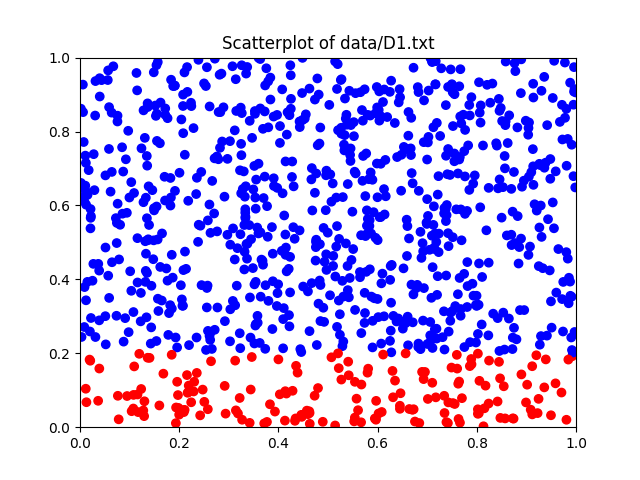
\includegraphics[width=0.6\linewidth]{D1plot.png}
            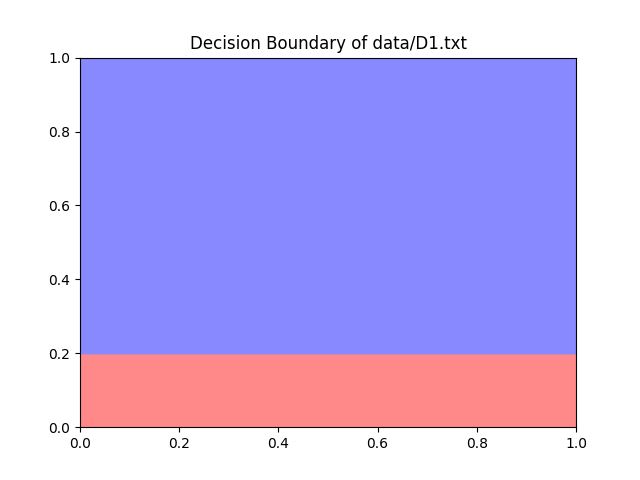
\includegraphics[width=0.6\linewidth]{D1region.png}
          \end{center}

          D2.txt:
          \begin{center}
            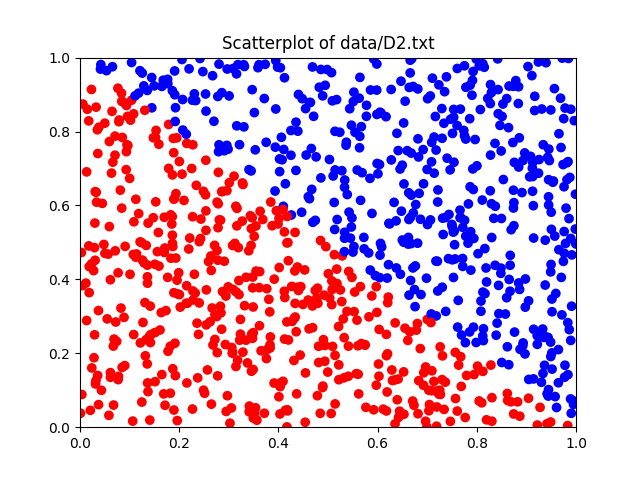
\includegraphics[width=0.6\linewidth]{D2plot.png}
            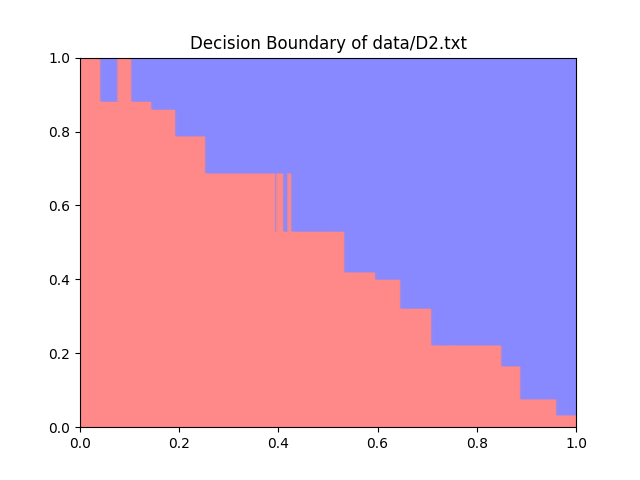
\includegraphics[width=0.6\linewidth]{D2region.png}
          \end{center}

          Conclusions: The true boundary of the data in \verb|D1.txt| is a horizontal line, but the true boundary of the data in \verb|D2.txt| is a diagonal line. Our decision tree only considers hypotheses that separate the data by axis-aligned lines, so the decision tree for \verb|D1.txt| only requires it takes many branches (zigzagging) to separate the data in \verb|D2.txt|.
        \end{soln}

\item (Learning curve)  [20 pts] We provide a data set Dbig.txt with 10000 labeled items.  Caution: Dbig.txt is sorted.
  \begin{itemize}

  \item You will randomly split Dbig.txt into a candidate training set of 8192 items and a test set (the rest).  Do this by generating a random permutation, and split at 8192.

  \item Generate a sequence of five nested training sets $D_{32} \subset D_{128} \subset D_{512} \subset D_{2048} \subset D_{8192}$ from the candidate training set.  The subscript $n$ in $D_n$ denotes training set size.  The easiest way is to take the first $n$ items from the (same) permutation above.  This sequence simulates the real world situation where you obtain more and more training data.

  \item For each $D_n$ above, train a decision tree.  Measure its test set error $err_n$.  Show three things in your answer: (1) List $n$, number of nodes in that tree, $err_n$. (2) Plot $n$ vs. $err_n$.  This is known as a learning curve (a single plot). (3) Visualize your decision trees' decision boundary (five plots). \\
  \end{itemize}

        \begin{soln}
          Number of nodes:
\begin{verbatim}
 n = 32
 nodes: 9
 err_n: 0.14767699115044253
 n = 128
 nodes: 19
 err_n: 0.09126106194690264
 n = 512
 nodes: 63
 err_n: 0.042588495575221264
 n = 2048
 nodes: 147
 err_n: 0.033738938053097356
 n = 8192
 nodes: 265
 err_n: 0.01382743362831862
\end{verbatim}

          Learning curve:
          \begin{center}
            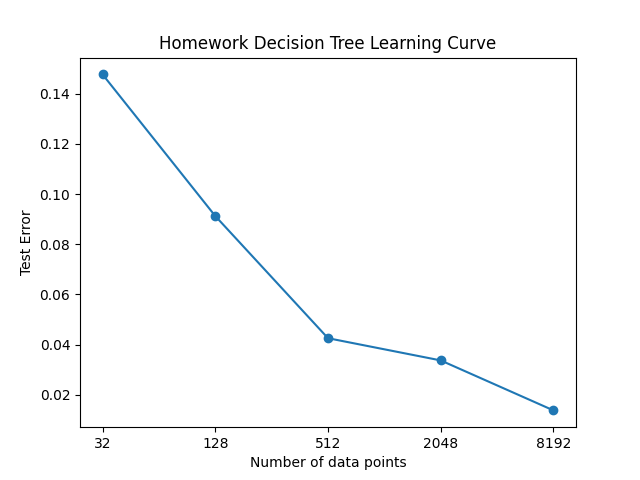
\includegraphics[width=0.6\linewidth]{DbigError.png}
          \end{center}

          Decision regions:
          \begin{center}
            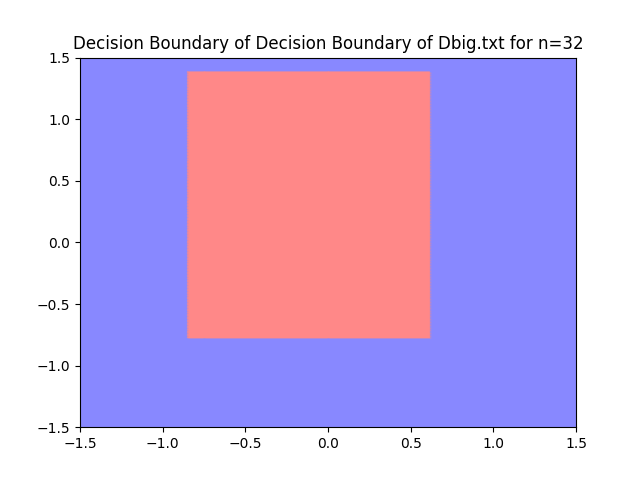
\includegraphics[width=0.6\linewidth]{DbigRegion32.png}
            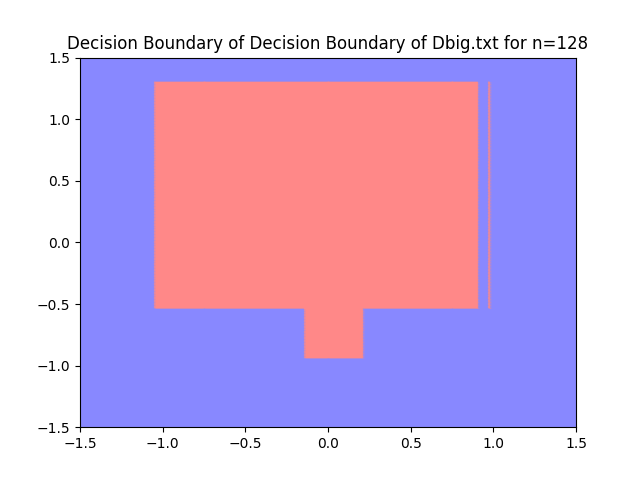
\includegraphics[width=0.6\linewidth]{DbigRegion128.png}
            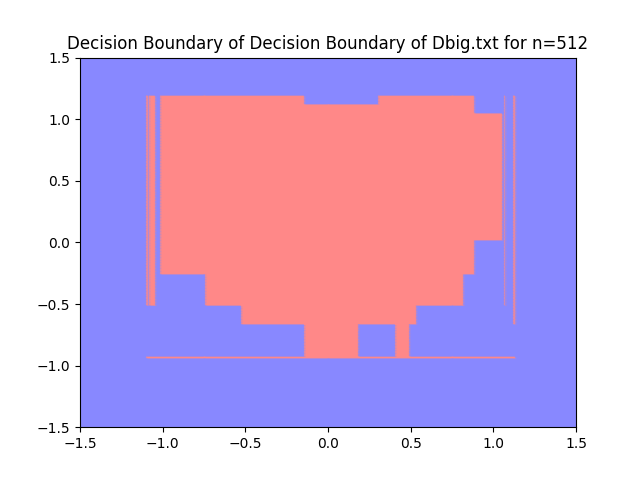
\includegraphics[width=0.6\linewidth]{DbigRegion512.png}
            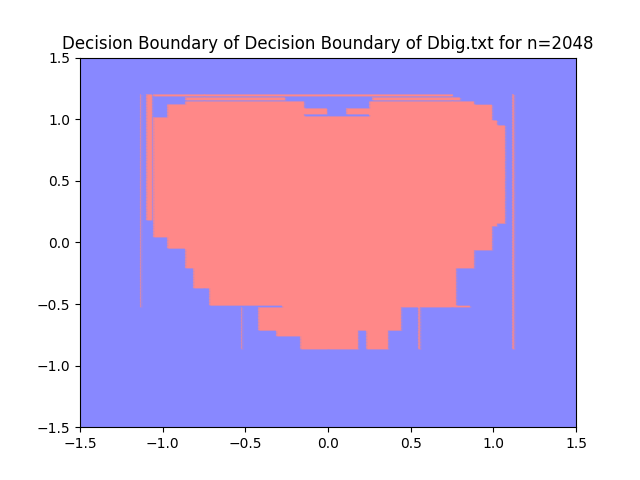
\includegraphics[width=0.6\linewidth]{DbigRegion2048.png}
            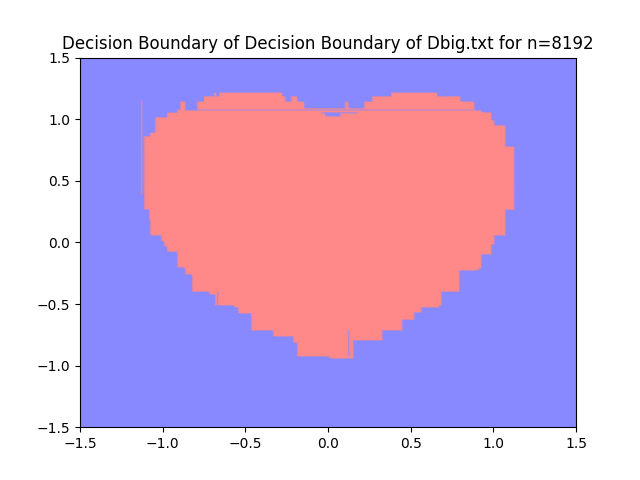
\includegraphics[width=0.6\linewidth]{DbigRegion8192.png}
          \end{center}
        \end{soln}

\end{enumerate}

\section{sklearn [10 pts]}
Learn to use sklearn (\url{https://scikit-learn.org/stable/}).
Use sklearn.tree.DecisionTreeClassifier to produce trees for datasets $D_{32}, D_{128}, D_{512}, D_{2048}, D_{8192}$.  Show two things in your answer: (1) List $n$, number of nodes in that tree, $err_n$. (2) Plot $n$ vs. $err_n$.

\begin{soln}
  Number of nodes:
\begin{verbatim}
 n = 32
 nodes: 7
 err_n: 0.14823008849557517
 n = 128
 nodes: 13
 err_n: 0.09292035398230092
 n = 512
 nodes: 47
 err_n: 0.05641592920353977
 n = 2048
 nodes: 113
 err_n: 0.020464601769911495
 n = 8192
 nodes: 231
 err_n: 0.014380530973451378
\end{verbatim}

  Learning curve:

  \begin{center}
    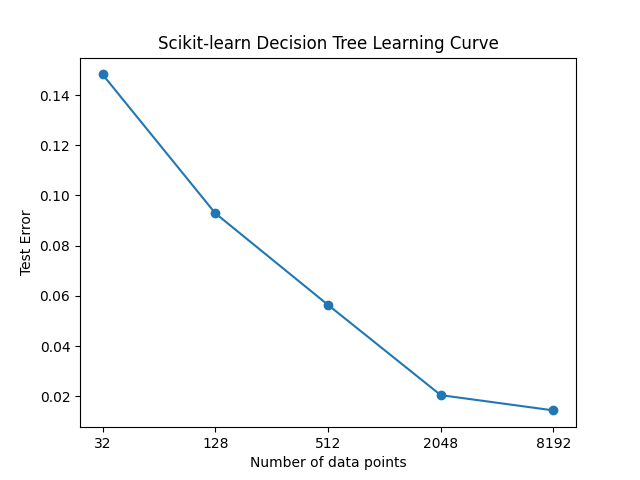
\includegraphics[width=0.6\linewidth]{SKLearnError.png}
  \end{center}

\end{soln}

\section{Lagrange Interpolation [10 pts]}
Fix some interval $[a, b]$ and sample $n = 100$ points $x$ from this interval uniformly. Use these to build a training set consisting of $n$ pairs $(x, y)$ by setting function $y = sin(x)$. \\

Build a model $f$ by using Lagrange interpolation, check more details in \url{https://en.wikipedia.org/wiki/Lagrange_polynomial} and \url{https://docs.scipy.org/doc/scipy/reference/generated/scipy.interpolate.lagrange.html}. \\

Generate a test set using the same distribution as your test set. Compute and report the resulting model’s train and test error. What do you observe?
Repeat the experiment with zero-mean Gaussian noise $\epsilon$ added to $x$. Vary the standard deviation for $\epsilon$ and report your findings.

\bibliographystyle{apalike}
\end{document}
